\chapter{Functors}
\label{chap:functors}

\epigraph{
  \term{Category} has been defined in order to be able to
  define \term{functor}...
}{---\textcite[18]{maclane-1998}}

In this chapter we explore functors and their relation to functors in
Haskell and Agda.

\section{Introduction}
\label{sec:functors-introduction}

\todo{What matters are the morphisms between categories, given by
  functors \parencite{marquis-2013}. A functor is a function between
  categories which maps objects to objects and morphisms to morphisms.
  Functors exists in both covariant and contravariant types. A functor
  is called covariant if it preserves the directions of arrows, and
  contravariant if it reverses the directions \todo{Cite MathWorld}.}

Mapping over lists, which is accomplished with the \texttt{map}
function, is a dominant idiom in Haskell \parencite{lipovaca-2011}.

The type signature of the \texttt{map} function is
\begin{codehaskell}
  map :: (a -> b) -> [a] -> [b]
\end{codehaskell}
According to the documentation of the Haskell Prelude, given a
function \texttt{f} and a list \texttt{xs}, \texttt{map f xs} is the
list obtained by applying \texttt{f} to each element in \texttt{xs}.
In other words,
\begin{codehaskell}
  map f [x1, x2, ..., xn] = [f x1, f x2, ..., f xn]
\end{codehaskell}
or, better,
\begin{codehaskell}
  map f [x1, x2, ...] = [f x1, f x2, ...]
\end{codehaskell}

The definition of the \texttt{map} function is
\begin{codehaskell}
  map :: (a -> b) -> [a] -> [b]
  map _ []     = []
  map f (x:xs) = f x : map f xs
\end{codehaskell}
Even though this is the correct definition of the \texttt{map}
function (it applies a function to all the elements of a list), it is
possible to implement alternative definitions. For instance,
\begin{codehaskell}
  map :: (a -> b) -> [a] -> [b]
  map _ []     = []
  map f (x:xs) = f x : f x : map f xs
\end{codehaskell}
This alternative \texttt{map} function applies a function to each
element in a list and duplicates each result.

Deciding whether the former or the latter \texttt{map} function is the
correct one for mapping over lists requires a more general approach.
This is achieved with the definition of the \texttt{Functor} type
class, which is used for types that can be mapped over and which
generalizes the \texttt{map} function as a \emph{uniform} action over
a parameterized type such as \texttt{[a]} in
\begin{codehaskell}
  (a -> b) -> [a] -> [b]
\end{codehaskell}

However, the defition of the \texttt{Functor} type class is not enough
to determine what a ``uniform action over a parameterized type'' is.
On the other hand, a comment in Haskell's documentation states that
all instances of the \texttt{Functor} type class \emph{should} satisfy
the functor laws. These laws, which are not part of the definition of
functors in Haskell, guarantee that a ``uniform action over a
parameterized type'' is actually uniform.

Functors in Haskell implement mathematical functors (that is, functors
in category theory) and the functor laws correspond to the conditions
that a mathematical functor \emph{must} satisfy in order to be a
functor. Studying mathematical functors may not be necessary for
uniformly mapping over a parameterized type, but it may be very useful
for better understanding what that means.

\section{Functors}
\label{sec:functors}

\todo{The definition of a functor is simpler (not as a concept, but as
  a definition) than the definition of a category. Our definition is
  based mainly on \cite{maclane-1998}, but some details were taken
  from \cite{poigne-1992}. Notation is different (ours is more
  explicit, which helps when comparing functors with functors in
  functional programming) (normally, the object and morphism functions
  have the same name). \cite{marquis-2013} is useful for informal
  definitions (the idea of preserving structure). \cite{eilenberg-maclane-1945}
  define functors on two arguments (covariant in one and contravariant
  in the other). The definition is pretty much the same ignoring the
  contravariant one (just for history). A covariant functor refers to
  functors as defined in this chapter: morphisms of categories that
  preserve domains and codomains. A contravariant functor, on the
  other side, refers to functors that reverse domains and codomains.
  The latter are not part of the definition in this chapter because
  they are not used (but they could with an implementation such as
  that of \parencite{elkins-2009}).}

\todo{Regarding examples, the power set and the identity functors are
  in almost any reference, but some of the others are based on
  \cite{poigne-1992}. It is important to remember that functors were
  just something necessary for defining natural transformations, which
  is not the case in functional programming.}

%% \parencites[13]{maclane-1998}[428]{poigne-1992}

\begin{definition}
  [Functor]

  \label{def:functor}

  \index{functor}

  Let \cat{C} and \cat{D} be categories\footnote{Whenever a category
    \cat{C} is mentioned, its sets of objects and morphisms, its
    domain and codomain functions, and its identity and composition
    functions (\catO{C} and \catM{C}, $\dom$ and $\cod$, and $\id$ and
    $\comp$, respectively) are implicitly mentioned as well. See
    Definition \ref{def:category}.}.
  A \term{functor}
  \begin{equation*}
    \label{eq:functor}
    \func{F}: \cat{C} \to \cat{D}
  \end{equation*}
  consists of an \term{object function}
  \begin{equation}
    \label{eq:functor-object}
    \funcO{F}: \catO{C} \to \catO{D}
  \end{equation}
  and a \term{morphism function}
  \begin{equation}
    \label{eq:functor-morphism}
    \funcM{F}: \catM{C} \to \catM{D}
    \text{,}
  \end{equation}
  which assigns to each morphism $f: a \to b \in \catM{C}$ a morphism
  \begin{equation*}
    \funcM{F}(f): \funcO{F}(a) \to \funcO{F}(b) \in \catM{D}
    \text{,}
  \end{equation*}
  such that, for all objects $a \in \catO{C}$,
  \begin{equation}
    \label{eq:functor-identity}
    \funcM{F}(\idO{a}) = \idO{\funcO{F}(a)}
    \text{,}
  \end{equation}
  and, whenever $g \comp f \in \catM{C}$,
  \begin{equation}
    \label{eq:functor-composition}
    \funcM{F}(g \comp f) = \funcM{F}(g) \comp \funcM{F}(f)
    \text{,}
  \end{equation}
  that is, such that the diagram in Figure
  \ref{fig:functor-composition} is commutative.
  \begin{figure}[htbp]
    \begin{center}
      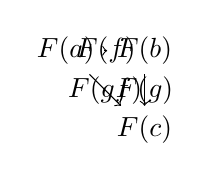
\begin{tikzpicture}
        \node (f a)                {$\funcO{F}(a)$};
        \node (f b) [right of=f a] {$\funcO{F}(b)$};
        \node (f c) [below of=f b] {$\funcO{F}(c)$};

        \draw [->] (f a) to node {$\funcM{F}(f)$} (f b);
        \draw [->] (f b) to node {$\funcM{F}(g)$} (f c);

        \draw [->] (f a) to node [swap] {$\funcM{F}(g \comp f)$} (f c);
      \end{tikzpicture}
    \end{center}
    \caption{}
    \label{fig:functor-composition}
  \end{figure}
\end{definition}

\begin{remark}
  \label{re:functor}

  Given two categories \cat{C} and \cat{D}, a functor $\func{F}:
  \cat{C} \to \cat{D}$ sends objects of \cat{C} to objects of \cat{D}
  and morphisms of \cat{C} to morphisms of \cat{D} in such a way that
  domains, codomains, identity morphisms, composite morphisms, and
  commutative diagrams are preserved. Functors are thus
  structure-preserving morphisms between categories
  \parencite[10]{marquis-2013}.
\end{remark}

\todo{Details... Really explain the diagram in the following remark.}

\begin{remark}
  \label{re:functor-picture}

  Given two categories \cat{C} and \cat{D}, a functor $\func{F}: \cat{C} \to \cat{D}$ may be thought
  of as giving a picture of all the objects and morphisms of \cat{C} in \cat{D} \parencite[16]{maclane-1998}.

  A functor \func{F} from \cat{C} to \cat{D} may be thought of as a
  picture of all the objects and morphisms of \cat{C} in \cat{D}. This
  may be represented by the commutative diagrams of Figure
  \ref{fig:functor}. The commutativity of the diagram in Figure
  \ref{fig:functor-b} is \eqref{eq:functor-composition}. Let $a$, $b$, and $c$
  be three objects in \cat{C}. Then there are three objects
  $\funcO{F}(a)$, $\funcO{F}(b)$, and $\funcO{F}(c)$ in \cat{D}, which
  are their pictures. Something similar happens with the morphisms in
  \cat{C}. Finally, a commutative diagram in \cat{C} is a commutative
  diagram in \cat{D} when mapping \cat{C} to \cat{D} with \func{F}.
  \begin{figure}[htb]
    \begin{subfigure}[b]{0.5\linewidth}
      \begin{center}
        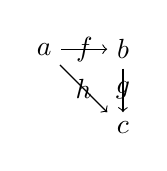
\begin{tikzpicture}
          \node (a)              {$a$};
          \node (b) [right of=a] {$b$};
          \node (c) [below of=b] {$c$};

          \draw [->] (a) to node        {$f$} (b);
          \draw [->] (b) to node        {$g$} (c);
          \draw [->] (a) to node [swap] {$h$} (c);
        \end{tikzpicture}
      \end{center}
      \caption{}
      \label{fig:functor-a}
    \end{subfigure}
    \begin{subfigure}[b]{0.5\linewidth}
      \begin{center}
        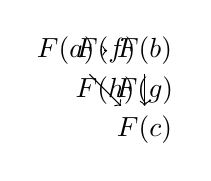
\begin{tikzpicture}
          \node (f a)                {$\funcO{F}(a)$};
          \node (f b) [right of=f a] {$\funcO{F}(b)$};
          \node (f c) [below of=f b] {$\funcO{F}(c)$};

          \draw [->] (f a) to node        {$\funcM{F}(f)$} (f b);
          \draw [->] (f b) to node        {$\funcM{F}(g)$} (f c);
          \draw [->] (f a) to node [swap] {$\funcM{F}(h)$} (f c);
        \end{tikzpicture}
      \end{center}
      \caption{}
      \label{fig:functor-b}
    \end{subfigure}
    \caption{$\func{F}: \cat{C} \to \cat{D}$ is a picture of \cat{C} in \cat{D}.}
    \label{fig:functor}
  \end{figure}
\end{remark}

\todo{Endofunctors are important for studying functors in Haskell and
  Agda.}

\begin{definition}
  \label{def:endofunctor}

  \index{endofunctor}

  An \term{endofunctor} is a functor from a category to itself.
\end{definition}

\todo{Bifunctors are important for studying algebras.}

\begin{definition}
  \label{def:bifunctor}

  \index{bifunctor}

  A \term{bifunctor}...
\end{definition}

\todo{Introduce examples?}

\begin{example}[Power set]

  \label{ex:functor-power-set}

  \index{power set}
  \index{functor!power set ---}

  The power set operation yields an endofunctor
  \begin{equation*}
    \func{P}: \set \to \set
    \text{.}
  \end{equation*}
  Its object function
  \begin{equation*}
    \funcO{P}: \catO{\set} \to \catO{\set}
  \end{equation*}
  is the power set operation. Given a set $X$, $\funcO{P}(X)$ is the
  set of all subsets of $X$, that is,
  \begin{equation}
    \label{eq:funcO-power-set}
    \funcO{P}(X) = \{S \mid S \subseteq X\}
    \text{.}
  \end{equation}
  Its morphism function
  \begin{equation*}
    \funcM{P}: \catM{\set} \to \catM{\set}
  \end{equation*}
  associates every function $f: X \to Y$ with a function
  $\funcM{P}(f): \funcO{P}(X) \to \funcO{P}(Y)$ such that
  \begin{equation}
    \label{eq:funcM-power-set}
    \funcM{P}(f)(S) = \{f(x) \mid x \in S\}
    \text{.}
  \end{equation}

  \begin{proof}
    \hfill
    \begin{itemize}
    \item
      \begin{align*}
        \funcM{P}(\idO{X})(S) & = \{\idO{X}(x) \mid x \in S\}\\
                              & = \{x \mid x \in S\}\\
                              & = S
      \end{align*}
      \begin{equation*}
        \idO{\funcO{P}(X)}(S) = S
      \end{equation*}
      \begin{equation*}
        \funcM{P}(\idO{X})(S) = \idO{\funcO{P}(X)}(S)
      \end{equation*}
    \item
      \begin{align*}
        \funcM{P}(g \comp f)(S) & = \{(g \comp f)(x) \mid x \in S \}\\
                                & = \{g(f(x)) \mid x \in S \}
      \end{align*}
      \begin{align*}
        (\funcM{P}(g) \comp \funcM{P}(f))(S)
          & = \funcM{P}(g)(\funcM{P}(f)(S))\\
          & = \funcM{P}(g)(\{f(x) \mid x \in S\})\\
          & = \{g(f(x)) \mid x \in S\}
      \end{align*}
      \begin{equation*}
        \funcM{P}(g \comp f)(S) = (\funcM{P}(g) \comp \funcM{P}(f))(S)
      \end{equation*}
    \end{itemize}
    \func{P} is a functor.
  \end{proof}

  \begin{note}
    The power set operation yields two functors on the category of
    sets (depending on how its action on morphisms is defined).
  \end{note}

\end{example}

\todo{In general, there are many functors between two given
  categories, and the question of how they are connected suggests
  itself. For instance, given a category C, there is always the
  identity functor from C to C which sends every object/morphism of C
  to itself. In particular, there is the identity functor over the
  category of sets. From Marquis. The nature of functors varies as
  much as that of categories. From Poigne-1992.}

\begin{example}[Identity]

  \label{ex:functor-identity}

  \index{identity}
  \index{functor!identity ---}

  Given a category \cat{C}, the identity functor from \cat{C} to
  \cat{C} sends every object/morphism of \cat{C} to itself.

  More precisely, an object function
  \begin{equation*}
    \funcO{I}: \catO{C} \to \catO{C}
  \end{equation*}
  defined as
  \begin{equation}
    \label{eq:funcO-id}
    \funcO{I}(a) = a
    \text{,}
  \end{equation}
  and a morphism function
  \begin{equation*}
    \funcM{I}: \catM{C} \to \catM{C}
  \end{equation*}
  defined as
  \begin{equation}
    \label{eq:funcM-id-b}
    \funcM{I}(f) = f
  \end{equation}
  yield a functor
  \begin{equation*}
    \func{I}: \cat{C} \to \cat{C}
    \text{.}
  \end{equation*}
  \begin{proof}
    \hfill
    \begin{itemize}
    \item
      Since
      \begin{equation*}
        \funcO{I}(a) = a
        \quad
        \text{and}
        \quad
        \funcM{I}(\idO{a}) = \idO{a}
        \text{,}
      \end{equation*}
      then
      \begin{equation*}
        \funcM{I}(\idO{a}) = \idO{\funcO{I}(a)}
        \text{.}
      \end{equation*}
    \item
      Since $\funcM{I}(f) = f$, $\funcM{I}(g) = g$, and
      $\funcM{I}(g \comp f) = g \comp f$ by the definition of
      $\funcM{I}$, then
      \begin{equation*}
        \funcM{I}(g \comp f) = \funcM{I}(g) \comp \funcM{I}(f)
        \text{.}
      \end{equation*}
    \end{itemize}
    As a consequence, \func{I} is a functor.
  \end{proof}

\end{example}

\todo{Some special kinds of functors, such as forgetful functors
  (which works for any set with structure) or inclusion functor are
  usually included in the list of examples, but they are not useful
  for this work.}

\begin{example}

  For each set $X$ we can construct the word monoid $X*$ with concatenation
  and empty word $\lambda$ as unit. Every mapping $f: X \to Y$ extends to a
  monoid homomorphism $f*: X* \to Y*$ by $f*(\epsilon) = \epsilon$ and
  $f*(vw) = f(v)f*(w)$ where $v$, $w \in X*$. These date define a functor
  $*: \catbf{Set} \to \catbf{Mon}$.
  Page 430. Poigné.

\end{example}

\begin{example}[Automata]

  \label{ex:functor-automata-1}

  \index{automata}

  $\func{U}: \catbf{Aut}(M) \to \catbf{Set}$ maps an $M$-automaton $(S,
  \delta)$ to $S$. A homomorphism $f: (S, \delta) \to (S', \delta')$ is
  defined by a function $f: S \to S'$ anyway.
  Page 430, Poigné.

\end{example}

\begin{example}[Automata]

  \label{ex:functor-automata-2}

  \index{automata}

  There are two functors in the other direction. $*: Set \to Aut(M)$ maps $X$
  to the automaton $X*$ with states $M \times X$ and transition function
  $\delta*: M \times (M \times X) \to M \times X$, $\delta*(m, (m', x)) =
  (m*m',x)$. Homomorphism $f*: X* \to Y*$ is defined by $f*(m,x) = (m,f(x))$.
  (Remark on the notation: we uniformly use the notation underscore$*$ for a
  certain kind of functors which we weill classify as free functors below. So
  the specific interpretation of for instance $X*$ depends on the context;
  here we refer to the 'free automaton' $X* = (M \times X, \delta*)$, in the
  context of monoids we refer to the word monoid $X* = (X*, conc, \epsilon)$.
  This should cause not too much confusion since the context will always be
  clearly stated, but has the merit of providing a uniform notation for a
  fundamental notion in mathematics.)

  The second functor $* : Set \to Aut(M)$ maps $X$ to the automaton $X_*$,
  with states $X^M$, and transition function $\delta*: M \times X^M \to X^M$,
  $\delta_*(m,g) = M \to X$ is defined by $\delta*(m,g)(m') = g(m*m')$. The
  homomorphism $f_*: X_* \to Y_*$ is defined by $f_*(g)(m) = f(g(m))$
  \parencite[430]{poigne-1992}.

\end{example}

\begin{example}

  \label{ex:functor-automata-3}

  \index{automata}
  Every $M$-automaton with transition function $\delta: M \times S \to S$
  defines a functor $D: M \to Set$ which maps the only object to $S$, and
  $D(x): S \to S$ is defined by $D(x)(s) = \delta(x,s)$
  \parencite[430]{poigne-1992}.

\end{example}

\begin{example}[Functions]

  \label{ex:functor-function}

  \index{discrete category}

  Given two discrete categories \cat{C} and \cat{D}, a functor
  $\func{F}: \cat{C} \to \cat{D}$ is a function.

  \begin{proof}
    \hfill
    \begin{itemize}
    \item
      Given a functor $\func{F}: \cat{C} \to \cat{D}$,
      \begin{equation*}
        f: \catO{C} \to \catO{D}
      \end{equation*}
      \begin{equation*}
        f(x) = \funcO{F}(x)
      \end{equation*}
    \item
      Given a function $f: C \to D$,
      \begin{equation*}
        \funcO{F}: C \to D
      \end{equation*}
      \begin{equation*}
        \funcO{F}(x) = f(x)
      \end{equation*}
      and
      \begin{equation*}
        \funcM{F}: \catM{C} \to \catM{D}
      \end{equation*}
      \begin{equation*}
        \funcM{F}(\idO{x}) = \idO{\funcO{F}(x)} = \idO{f(x)}
      \end{equation*}

      \begin{proof}
        The definition of \funcM{F} gives the first law of functors, and the
        second law is trivial because the only morphisms on the categories are
        identities.
      \end{proof}
    \end{itemize}
  \end{proof}

\end{example}

\begin{example}[List]

  \label{ex:functor-list}

  The functor $List: \catbf{Set} \to \catbf{Set}$ maps a set $X$ to the
  list $X*$. The function $List(f)(x_1...x_n) = f(x_1)...f(x_n)$ is
  known as 'maplist' in programming.
  Relate to examples
  \ref{ex:functor-list-haskell} and \ref{ex:functor-list-agda}
  \parencite[431]{poigne-1992}.

\end{example}

\begin{example}

  Cartesian products of sets define a functor $\times : Set \times Set \to Set$.
  A pair $(X,Y)$ of sets is mapped to its Cartesian product, and a pair
  $(f: X \to Y, g: X' \to Y')$ of functions to the function
  $f \times g: X \times X' \to Y \times Y'$ such that
  $f \times g(x,x') = (f(x),g(x'))$ \parencite[431]{poigne-1992}.

\end{example}

\begin{example}

  Function space functors from Poigné. Relate to examples
  {ex:functor-function-haskell} and {ex:functor-function-agda}.

\end{example}

\section{Functors in Haskell}
\label{sec:functors-haskell}

  \todo{For functors in Haskell:
    \cite{lipovaca-2011,osullivan-2008,yorgey-2009}. \todo{Add the
      Haskell Wikibook, HaskellWiki}. A different approach to that of
    this chapter and the Typeclassopedia is the one used by
    \parencite{elkins-2009}.}

\todo{Ideas from \parencite{yorgey-2009}: The Functor type class is
  the most ubiquitous type class in the Haskell libraries. A simple
  intuition is that it represents a ``container'' of some sort, along
  with the ability to apply a function uniformly to every element in
  the container. Another intuition is that it represents some sort of
  ``computational context.'' This is generally more useful, but more
  difficult to explain (more general). These should be clarified by
  the examples. There are many examples that don't exactly fit either
  of the above intuitions.}

Functors in Haskell are defined by the \texttt{Functor} type class,
which is exported by the Haskell Prelude:
\index{\texttt{Functor}}
\begin{codehaskell}
  class Functor f where
    fmap :: (a -> b) -> f a -> f b
\end{codehaskell}
It is used for types that can be mapped over, and generalizes the
\texttt{map} function on lists with a uniform action over a
parameterized type.

\todo{Idea from \parencite{lipovaca-2011}: A functor is for types that
  can be mapped over.}

\todo{Idea from \parencite{lipovaca-2011}: The f a and f b in the type
  signature for fmap tell us that f isn't just a type; it is a type
  constructor which takes another type as parameter. A more precise
  way to say this is that the kind of f must be... For example,
  Maybe.}

\todo{Idea from \parencite{yorgey-2009}: From the container point of
  view, fmap applies a function to each element of a container,
  without altering the structure of the container. From the context
  point of view, the intention is that fmap applies a function to a
  value without altering its context.}

It is important to note that \texttt{f} is a type constructor rather
than a type (its kind is \texttt{* -> *} and not \texttt{*}).
\texttt{[]} and \texttt{Maybe} are examples of such type constructors.
The result of applying a type constructor to a type (for example,
\texttt{Int} or \texttt{Bool}) is a type or concrete type (that is,
something of kind \texttt{*}). Therefore, the kinds of \texttt{[] Int}
(that is, \texttt{[Int]}) and \texttt{Maybe Int} are both \texttt{*}.
As another example, since the kind of \texttt{Either} is \texttt{* ->
  * -> *}, it can not be declared as an instance of the
\texttt{Functor} type class. However, a type constructor can be
partially applied and something like \texttt{Either a} can be declared
as an instance of \texttt{Functor}.

The fact that \texttt{f} is a type constructor can be made explicit
using the language option \texttt{KindSignatures}:
\begin{codehaskell}
  class Functor (f :: * -> *) where
    fmap :: (a -> b) -> f a -> f b
\end{codehaskell}
The kind signature of \texttt{f} shows that it corresponds to the
object function of a mathematical functor \eqref{eq:functor-object}: it sends
objects of \hask (types) to objects of \hask (types).

Also, \texttt{fmap} is curried and can be rewritten with extra and
unnecessary parentheses for emphasis:
\begin{codehaskell}
  class Functor (f :: * -> *) where
    fmap :: (a -> b) -> (f a -> f b)
\end{codehaskell}
The type of \texttt{fmap} shows that it corresponds to the morphism
function of a mathematical functor \eqref{eq:functor-morphism}: it sends
morphisms of \hask (functions) to morphisms of \hask (functions).

\todo{Summary from \parencite{elkins-2009}: Functors are mappings
  between categories. In Haskell, instances of the Functor type class
  correspond to functors from \hask to \hask. The type constructor is
  the action on objects, and fmap is the action on morphisms.}

%% Intuition from the Typeclassopedia: There are two fundamental ways to think
%% about fmap. The first has already been touched on: it takes two parameters, a
%% function and container, and applies the function inside the ``container'',
%% producing a new container. Alternately, we can think of fmap as applying a
%% function to a value in a context (without altering the context).

%% Just like all other Haskell functions of ``more than one parameter,'' however,
%% fmap is actually curried: it does not really take two parameters, but takes a
%% single parameter and returns a function. For emphasis, we can write fmap's
%% type with extra parentheses. Written in this form, it is apparent that fmap
%% transforms a ``normal'' function into one which operates over
%% containers/contexts. This transformation is often referred to as a lift; fmap
%% ``lifts'' a function from the ``normal world'' into the ``f world.''

%% More from Learn You...: ``Give me a function that takes an a and returns a b
%% and a box with an a (or several of them) inside it, and I'll give you a box
%% with a b (or several of them) inside it.'' It applies the function to the
%% element inside the box.

%% ...: We can also look at functor values as values with an added context. For
%% instance, Maybe values have the extra context that they might have failed.
%% With lists, the context is that the value can actually be several values at
%% once or none. fmap applies a function to the value while preserving its
%% context.

%% ...: If we want to make a type constructor an instance of Functor, it must
%% have a kind of * -> *, which means that it takes exactly one concrete type as
%% a type parameter.

%% ...: If we write fmap :: (a -> b) -> (f a -> f b), we can think of fmap not as
%% a function that takes one function and a functor value and returns a functor
%% value, but as a function that takes a function and returns a new function
%% that's just like the old one, except that it takes a functor value as a
%% parameter and returns a functor value as the result. It takes an a -> b
%% function and returns a function f a -> f b. This is called lifting a function.

%% ...: You can think of fmap in two ways: - As a function that takes a function
%% and a functor value and then maps that function over the functor value. - As a
%% function that takes a function and lifts that function so it operates on
%% functor values. Both views are correct.

%% RWH: We can think of fmap as a kind of lifting function. It takes a function
%% over ordinary values a -> b, and lifts it to become a function over containers
%% f a -> f b, where f is the container type.

%% ...: The definition of Functor imposes a few obvious restrictions on what we
%% can do with fmap. For example, we can only make instances of Functor from
%% types that have exactly one type parameter. In addition, we can't place any
%% constraints on our type definition.

%% ...: We've make a few implicit assumptions about how functors ought to work.
%% It's jelpful to make these explicit and to think of them as rules to follow,
%% because this lets us treat functors as uniform, well-behaved objects. We have
%% only two rules to remember, and they're simple: - Out first rule is functors
%% must preserve identity. That is, applying fmap id to a value should give us
%% back an identical value. - Our second rule is functors must be composable.
%% That is, composin two uses of fmap should give the same result as one fmap
%% with the same functions composed.

%% ...: Another way of looking at these two rules is that functors must preserve
%% shape. The structure of a collection should not be affected by a functor; only
%% the values that it contains should change.

%% ...: If you're writing a Functor instance, it's useful to keep these rules in
%% mind, and indeed to test them, because the compiler can't check the rules
%% we've just listed. On the other hand, if you're simply using functors, the
%% rules ``natural'' enough that there's no need to memorize them. They just
%% formalize a few intuitive notions of ``do what I mean.''

%% The Prelude says that a functor should obey the following laws.

%% As far as the Haskell language itself is concerned, the only requirement to be
%% a Functor is an implementation of fmap with the proper type. Any sensible
%% Functor instance, however, will also satisfy the functor laws, which are part
%% of the definition of a mathematical functor. There are two; together, these
%% laws ensure that fmap f does not change the structure of a container, only the
%% elements. Equivalently, and more simply, they ensure that fmap f changes a
%% value without altering its context. From the typeclassopedia.

%% Haskell does not enforce the laws, a functor can be defined and it does not have
%% to obey the functor laws in order to be a Haskell functor. The laws can be defined
%% informally and mentally checked.

%% The first law:

Although Haskell's documentation states that functors \emph{should}
obey the functor laws, this is not mandatory when declaring an instance
of the \texttt{Functor} type class.

The first law can be stated as:
\begin{codehaskell}
  fmap id = id
\end{codehaskell}
Polymorphism in Haskell allows to write just \texttt{id} in both sides of this
law, but the types of each \texttt{id} are different (which is more
obvious when comparing this with \eqref{eq:functor-identity}). A more precise way
of stating the first law in Haskell follows:
\begin{codehaskell}
  fmap (id :: a -> a) = (id :: f a -> f a)
\end{codehaskell}

%% Typeclassopedia: The first law says that mapping the identity function over
%% every item in a container has no effect.

The second law can be stated as:
\begin{codehaskell}
  fmap (g . f) = fmap g . fmap f
\end{codehaskell}
This law corresponds to \eqref{eq:functor-composition}.

Proving both of these laws amounts to proving \eqref{eq:functor-identity} and
\eqref{eq:functor-composition}.

%% Typeclassopedia: The second says that mapping a composition of two functions
%% over every item in a container is the same as first mapping one function, and
%% then mapping the other.

%% The instances found on the standard library obey these rules, but they will be
%% checked in this chapter.

%% Typeclass...: Technically, these laws make f and fmap together an endofunctor
%% on Hask, the category of Haskell types (ignoring bottom, which is a party
%% pooper).

%% Learn You: All functors are expected to exhibit certain kind of properties and
%% behaviors. They should reliably behave as things that can be mapped over.
%% Calling fmap on a functor should just map a function over the
%% functor---nothing more. This behavior is described by the functor laws. All
%% instances of Functor should abide by these two laws. They aren't enforced by
%% Haskell automatically, so you need to test them yourself when you make a
%% functor. All the Functor instances in the standard library obey these laws.

%% ...: 1: The first functor law states that if we map the id function over a
%% functor value, the functor value that we get back should be the same as the
%% original functor value. Written a bit more formally, it means that fmap id =
%% id. So essentially, this says that if we do fmap id over a functor value, it
%% should be the same as just applying it to the value. If we view the functor
%% value as something that can be mapped over, the fmap id = id law seems kind of
%% trivial or obvious.

%% ...: 2: The second law says that composing two functions and then mapping the
%% resulting function over a functor should be the same as first mapping one
%% function over the functor and then mapping the other one. Formally written,
%% that means fmap (f . g) = fmap f . fmap g. Or to write it in another way, for
%% any functor value x, the following should hold: fmap (f . g) x = fmap f (fmap
%% g x).

%% If we can show that some type obeys both functor laws, we can rely on it
%% having the same fundamental behaviors as other functors when it comes to
%% mapping. We can know that when we use fmap on it, there won't be anything
%% other than mapping going on behind the scenes and that it will act like a
%% thing that can be mapped over---that is, a functor.

%% ...: Be sure that you understand how function composition works. Many times,
%% you can intuitively see how these laws hold because the types act like
%% containers or functions. You can also try them on a bunch of different values
%% of a type and be able to say with some certainty that a type does indeed obey
%% the laws.

\begin{note}
  A different approach is that of \parencite{jeuring-2012}, which
  includes the implementation of a library for testing the laws of
  type classes such as \texttt{Functor}.
\end{note}

\todo{Move on to examples of functors in Haskell.}

\begin{example}
  \label{ex:functor-identity-haskell}
  \hfill
  \begin{figure}[htbp]
    \begin{codehaskell}
instance Functor Identity where
  fmap f (Identity x) = Identity (f b)
    \end{codehaskell}
    \caption{}
    \label{fig:functor-identity-haskell}
  \end{figure}
\end{example}

\begin{example}[\texttt{Maybe}]
  \label{ex:functor-maybe-haskell}

  \index{\texttt{Maybe}}
  \index{\texttt{Functor}!\texttt{Maybe}}

  When declaring an instance of the \texttt{Functor} type class, it is
  necessary to define a type constructor and to implement an
  appropiate \texttt{fmap} for that particular type constructor.

  Given a type constructor \texttt{f}, the type signature of
  \texttt{fmap} is:
  \begin{codehaskell}
    fmap :: Functor f => (a -> b) -> f a -> f b
  \end{codehaskell}
  In the case of the \texttt{Maybe} type constructor, replacing the
  \texttt{f}'s in the type signature of \texttt{fmap} gives the type
  signature of the function we need to define in order to make it an
  instance of the \texttt{Functor} type class:
  \begin{codehaskell}
    fmap :: (a -> b) -> Maybe a -> Maybe b
  \end{codehaskell}

  \begin{equation}
    \label{eq:maybe-fmap-nothing}
    \text{\texthaskell{fmap \_ Nothing = Nothing}}
  \end{equation}
  \begin{equation}
    \label{eq:maybe-fmap-just}
    \text{\texthaskell{fmap f (Just x) = Just (f x)}}
  \end{equation}

  The definition of the \texttt{Maybe} functor is:

  \begin{figure}[htbp]
    \begin{codehaskell}
    instance Functor Maybe where
      fmap _ Nothing  = Nothing
      fmap f (Just x) = Just (f x)
    \end{codehaskell}
    \caption{}
    \label{fig:functor-maybe-haskell}
  \end{figure}

The Maybe type constructor represents a container which might hold a
single element. Under the context point of view, it represents a
context with possible failure \parencite{yorgey-2009}. It is like a box
that can hold nothing, or it can contain one item
\parencite{lipovaca-2011}. The instance for Maybe shows
clearly what fmap needs to do \parencite{osullivan-2008}.

Two different intuitions are usually presented when explaining the
\texttt{Maybe} functor. From a container point of view, the
\texttt{Maybe} type constructor represents a container which might
hold a single element. If this container actually holds a single
element, \texttt{fmap} applies a given function to it. Otherwise, it
does nothing. From a context point of view, it represents a context
with possible failure (in the case of \texttt{Nothing}). A third
intuition is more appropiate when comparing an instance of the
\texttt{Functor} type class with mathematical functors: if there is a
function \texttt{f :: a -> b}, \texttt{fmap} \emph{lifts} that
function and the result is a function which can be used in the
container or context world (in this case, a function with \texttt{f a
  -> f b} as type signature).

Although some familiarity with \texttt{Maybe} as an instance of the
\texttt{Functor} type class makes it easy to see that it is in fact a
functor, it is possible to prove \eqref{eq:functor-identity} and
\eqref{eq:functor-composition} in order to demonstrate that \texttt{Maybe} and
its implementation of \texttt{fmap} actually constitute a functor.

  \begin{proof}
    We shall prove \eqref{eq:functor-identity} and \eqref{eq:functor-composition}:
    \begin{itemize}
    \item
      For proving the first law, there are two cases: \texttt{Nothing}
      and \texttt{Just x}. In the case of a \texttt{Nothing}:
      \begin{steps}
        \steph{fmap id Nothing}
          \eqbydefh{fmap}
        \steph{Nothing}
          \eqbydefh{id}
        \steph{id Nothing}
      \end{steps}
      And in the case of a \texttt{Just x}:
      \begin{steps}
        \steph{fmap id (Just x)}
          \eqbydefh{fmap}
        \steph{Just (id x)}
          \eqbydefh{id}
        \steph{Just x}
          \eqbydefh{id}
        \steph{id (Just x)}
      \end{steps}
      So \texttt{fmap id = id}.
    \item
      Similarly, there are two cases for proving the second law. For
      \texttt{Nothing}:
      \begin{steps}
        \steph{(fmap g . fmap f) Nothing}
          \eqbydefh{(.)}
        \steph{fmap g (fmap f Nothing)}
          \eqbydefh{fmap}
        \steph{fmap g Nothing}
          \eqbydefh{fmap}
        \steph{Nothing}
          \eqbydefh{fmap}
        \steph{fmap (g . f) Nothing}
      \end{steps}
      And for \texttt{Just x} (in this case, it is easier to prove that
      both sides of the second law are \texttt{Just (g (f x))}):
      \begin{steps}
        \steph{fmap (g . f) (Just x)}
          \eqbydefh{fmap}
        \steph{Just ((g . f) x)}
          \eqbydefh{(.)}
        \steph{Just (g (f x))}
      \end{steps}
      Finally:
      \begin{steps}
        \steph{(fmap g . fmap f) (Just x)}
          \eqbydefh{(.)}
        \steph{fmap g (fmap f (Just x))}
          \eqbydefh{fmap}
        \steph{fmap g (Just (f x))}
          \eqbydefh{fmap}
        \steph{Just (g (f x))}
      \end{steps}
      So \texttt{fmap (g . f) = fmap g . fmap f}.
    \end{itemize}
    The \texttt{Maybe} type constructor and \texttt{fmap} thus
    define a real functor because they satisfy both laws.
  \end{proof}
\end{example}

\begin{example}[\texttt{[]}]
  \label{ex:functor-list-haskell}

  \index{\texttt{[]}}
  \index{\texttt{Functor}!\texttt{[]}}
  The type signature of \texttt{fmap} for the list type constructor
  (\texttt{[]}) is:
  \begin{codehaskell}
    fmap :: (a -> b) -> [a] -> [b]
  \end{codehaskell}

  Haskell defines this instance as:
  \begin{codehaskell}
    instance Functor [] where
      fmap = map
  \end{codehaskell}
  However, it is possible to implement \texttt{fmap} without using
  \texttt{map}, as shown in Figure \ref{fig:functor-list-haskell}.
  \begin{figure}[htbp]
    \begin{codehaskell}
    instance Functor [] where
      fmap _ []     = []
      fmap f (x:xs) = f x : fmap f xs
    \end{codehaskell}
    \caption{}
    \label{fig:functor-list-haskell}
  \end{figure}

  According to \parencite{yorgey-2009}, the usual argument for
  having \texttt{map} as a separate function in Haskell is that
  ``someone using Haskell, when using \texttt{map} incorrectly, would
  much rather see an error about lists than about functors.''

  There are three correct ways of thinking about the \texttt{[]}
  functor:
  \begin{itemize}
  \item
    Under the container point of view, a list is a container or a box and
    \texttt{fmap} is used for applying a function to each element of the
    list.
  \item
    Under the context point of view, a list represents a single value
    which is nondeterministically chosen from among several
    possibilities (the elements of the list) and the list functor
    represents a context of nondeterministic choice
    \parencite{yorgey-2009}.
  \item
    And the intuition which best suits the spirit of mathematical
    functors is that \texttt{fmap} \emph{lifts} a function. A function
    \texttt{f :: a -> b} can not be applied to a list of \texttt{a}
    (\texttt{[a]}), but \texttt{fmap f :: [a] -> [b]} can.
  \end{itemize}

  \begin{proof}
    Both laws are proven by induction:
    \begin{itemize}
    \item
      The basis case for the first law is:
      \begin{steps}
        \steph{fmap id []}
          \eqbydefh{fmap}
        \steph{[]}
          \eqbydefh{id}
        \steph{id []}
      \end{steps}
      The induction step, which uses \texttt{fmap id xs = xs} as
      inductive hypothesis, is:
      \begin{steps}
        \steph{fmap id (x:xs)}
          \eqbydefh{fmap}
        \steph{id x : fmap id xs}
          \eqbydefh{id}
        \steph{x : fmap id xs}
          \eqbyihh
        \steph{x:xs}
          \eqbydefh{id}
        \steph{id (x:xs)}
      \end{steps}
    \item
      For the second law, the basis case is:
      \begin{steps}
        \steph{(fmap g . fmap f) []}
          \eqbydefh{(.)}
        \steph{fmap g (fmap f [])}
          \eqbydefh{fmap}
        \steph{fmap g []}
          \eqbydefh{fmap}
        \steph{[]}
          \eqbydefh{fmap}
        \steph{fmap (g . f) []}
      \end{steps}
      The induction case (with
      \begin{codehaskell}
        fmap (g . f) xs = (fmap g . fmap f) xs
      \end{codehaskell}
      as inductive hypothesis) proves that both sides of
      the second law are
      \begin{codehaskell}
        g (f x) : (fmap g . fmap f) xs
      \end{codehaskell}
      For the left side:
      \begin{steps}
        \steph{fmap (g . f) (x:xs)}
          \eqbydefh{fmap}
        \steph{(g . f) x : fmap (g . f) xs}
          \eqbydefh{(.)}
        \steph{g (f x) : fmap (g . f) xs}
          \eqbyihh
        \steph{g (f x) : (fmap g . fmap f) xs}
      \end{steps}
      And for the right side:
      \begin{steps}
        \steph{(fmap g . fmap f) (x:xs)}
          \eqbydefh{(.)}
        \steph{fmap g (fmap f (x:xs))}
          \eqbydefh{fmap}
        \steph{fmap g (f x : fmap f xs)}
          \eqbydefh{fmap}
        \steph{g (f x) : fmap g (fmap f xs)}
          \eqbydefh{(.)}
        \steph{g (f x) : (fmap g . fmap f) xs}
      \end{steps}
    \end{itemize}
    So \texttt{[]} and \texttt{fmap} (or \texttt{map}) satisfy the
    functor laws and hence constitute one.
  \end{proof}
\end{example}

\begin{example}[\texttt{((,) a)}]
  \label{ex:functors-haskell-product}
  \index{\texttt{Product}}
  \index{\texttt{Functor}!\texttt{Product}}
  Since the kind of \texttt{(,)} is \texttt{* -> * -> *}, it can be
  partially applied in order to define an instance of the
  \texttt{Functor} type class for it. Given a concrete type
  \texttt{a}, the type signature of \texttt{fmap} for \texttt{((,) a)}
  is:
  \begin{codehaskell}
    fmap :: (b -> c) -> (a, b) -> (a, c)
  \end{codehaskell}

  The \texttt{((,) a)} functor is defined as follows:
  \begin{codehaskell}
    instance Functor ((,) a) where
      fmap f (x, y) = (x, f y)
  \end{codehaskell}
  Note that this the only way of defining \texttt{fmap} (regardless of
  the functor laws and within ``platonic'' \hask).

  \texttt{((,) a)} represents a container which holds an annotation of
  type \texttt{a} along with the actual value it holds
  \parencite{yorgey-2009}. The first element of a tuple is never
  modified by \texttt{fmap}, it is fixed.

  \todo{Is there a better way to say ``annotation''?}

  \begin{proof}
    \hfill
    \begin{itemize}
    \item
      The following reasoning proves the first law:
      \begin{steps}
        \steph{fmap id (x, y)}
          \eqbydefh{fmap}
        \steph{(x, id y)}
          \eqbydefh{id}
        \steph{(x, y)}
          \eqbydefh{id}
        \steph{id (x, y)}
      \end{steps}
    \item
      The second law is proven in a similar way:
      \begin{steps}
        \steph{(fmap h . fmap g) (x, y)}
          \eqbydefh{(.)}
        \steph{fmap h (fmap g (x, y))}
          \eqbydefh{fmap}
        \steph{fmap h (x, g y)}
          \eqbydefh{fmap}
        \steph{(x, h (g y))}
          \eqbydefh{(.)}
        \steph{(x, (h . g) y)}
          \eqbydefh{fmap}
        \steph{fmap (h . g) (x, y)}
      \end{steps}
    \end{itemize}
    The above reasonings prove that the functor laws hold for the
    \texttt{((,) a)} type constructor and its implementation of
    \texttt{fmap}.
  \end{proof}
\end{example}

\begin{example}[\texttt{Either a}]

  \label{ex:functor-either-haskell}

  \index{\texthaskell{Either}}
  \index{\texttt{Functor}!\texttt{Either}}

  The \texttt{Either} type constructor takes two type parameters. It
  is thus possible to declare \texttt{Either a} as an instance of the
  \texttt{Functor} type class. The type signature of \texttt{fmap} for
  a concrete type \texttt{a} is:
  \begin{codehaskell}
    fmap :: (b -> c) -> Either a b -> Either a c
  \end{codehaskell}

  The instance is defined as follows:
  \begin{codehaskell}
    instance Functor (Either a) where
      fmap _ (Left x)  = Left x
      fmap g (Right y) = Right (g y)
  \end{codehaskell}
  This is similar to the \texttt{((,) a)} functor in that there is
  only one way of implementing \texttt{fmap} (again, regardless of the
  functor laws and within ``platonic'' \hask).

  \texttt{Either a b} represents a container which can have either a
  value of type \texttt{a} (which usually represents some sort of
  error condition) or a value of type \texttt{b}. It is very similar
  to \texttt{Maybe} in that it represents possible failure, but it can
  carry some additional information about the failure
  \parencite{yorgey-2009}.

  The behavior of \texttt{fmap} is practically the same as the
  behavior of \texttt{fmap} for \texttt{Maybe}: a given function is
  mapped in the case of a \texttt{Right}, but not in the case of a
  \texttt{Left}. The \texttt{Left} is like an empty box or container
  (like \texttt{Nothing}) with an error message written on the side
  which explains why it is empty \parencite{lipovaca-2011}.

  \begin{proof}
    Proving that \texttt{Either a} is a functor is very similar to
    proving that \texttt{Maybe} is a functor.
    \begin{itemize}
    \item
      In the case of a \texttt{Left} constructor, the first law is
      proven as follows:
      \begin{steps}
        \steph{fmap id (Left x)}
          \eqbydefh{fmap}
        \steph{Left x}
          \eqbydefh{id}
        \steph{id (Left x)}
      \end{steps}
      In the case of a \texttt{Right} constructor, the following
      reasoning proves the first law:
      \begin{steps}
        \steph{fmap id (Right y)}
          \eqbydefh{fmap}
        \steph{Right (id y)}
          \eqbydefh{id}
        \steph{Right y}
          \eqbydefh{id}
        \steph{id (Right y)}
      \end{steps}
    \item
      For the second law and a \texttt{Left}, we have:
      \begin{steps}
        \steph{(fmap h . fmap g) (Left x)}
          \eqbydefh{(.)}
        \steph{fmap h (fmap g (Left x))}
          \eqbydefh{fmap}
        \steph{fmap h (Left x)}
          \eqbydefh{fmap}
        \steph{Left x}
          \eqbydefh{fmap}
        \steph{fmap (h . g) (Left x)}
      \end{steps}
      And for a \texttt{Right}:
      \begin{steps}
        \steph{(fmap h . fmap g) (Right y)}
          \eqbydefh{(.)}
        \steph{fmap h (fmap g (Right y))}
          \eqbydefh{fmap}
        \steph{fmap h (Right (g y))}
          \eqbydefh{fmap}
        \steph{Right (h (g y))}
          \eqbydefh{(.)}
        \steph{Right ((h . g) y)}
          \eqbydefh{fmap}
        \steph{fmap (h . g) (Right y)}
      \end{steps}
    \end{itemize}
    In conclusion, the \texttt{Either a} type constructor is a
    functor.
  \end{proof}
\end{example}

\begin{example}[\texttt{((->) a)}]
  \label{ex:functors-haskell-function}
  \index{\texttt{Function}}
  \index{\texttt{Functor}!\texttt{Function}}
  Declaring \texttt{((->) a)} as an instance of the \texttt{Functor}
  type class is an interesting example. Its type signature for
  \texttt{fmap} is:
  \begin{codehaskell}
    fmap :: (b -> c) -> (a -> b) -> a -> c
  \end{codehaskell}
  This type signature is exactly the same as that of \texttt{(.)}
  (that is, function composition). As a consequence, the instance
  declaration is:
  \begin{codehaskell}
    instance Functor ((->) a) where
      fmap g f = \x -> g (f x)
  \end{codehaskell}
  An equivalent way of defining this instance is:
  \begin{codehaskell}
    instance Functor ((->) a) where
      fmap = (.)
  \end{codehaskell}

%%   The Typeclassopedia: ((->) e), the type of functions which take a value of
%%   type e as parameter, is a Functor. It would be clearer to write it as (e
%%   ->), but that syntax is not allowed. However, you can certainly think of it
%%   as (e ->). As a container, (e -> a) represents a (possibly infinite) set of
%%   values of a, indexed by values of e. Alternatively, and more usefully, (e
%%   ->) can be thought of as a context in which a value of type e is available
%%   to be consulted in a read-only fashion. This is also why ((->) e) is
%%   sometimes referred to as the reader monad.

%%   Learn You...: Functions as functors: Another instance of Functor that we've
%%   been dealing with all along is (->) r. The function type r -> a can be
%%   rewritten as (->) r a. It's just a type constructor that takes two type
%%   parameters, like Either. From Control.Monad.Instances.

%% Learn You: Function composition! We pipe the output of r -> a into the input
%% of a -> b to get a function r -> b, which is exactly what function composition
%% is all about. Another way to write it: fmap = (.)
%% fmap (*3) (+100) 1 = 303

%% ...: Just like all functors, functions can be thought of as values with
%% contexts. When we have a function like (+3), we can view the value as the
%% eventual result of the function, and the context is that we need to apply the
%% function to something to get to the result. Using fmap (*3) on (+100) will
%% create another function that acts like (+100), but before producing a result,
%% (*3) will be applied to that result.

%% ...: The fact that fmap is function composition when used on functions isn't
%% so terribly useful right now, but at least it's very interesting. It also
%% bends our minds a bit and lets us see how things that act more like
%% computations than boxes can be functors. The function being mapped over a
%% computation results in the same sort of computation, but the result of that
%% computation is modified with the function.

  \begin{proof}
    \hfill
    \begin{itemize}
    \item
      The first law is proven as follows:
      \begin{steps}
        \steph{fmap id f}
          \eqbydefh{fmap}
        \steph{id . f}
          \eqbyh{identity of \texthaskell{(.)}}
        \steph{f}
          \eqbydefh{id}
        \steph{id f}
      \end{steps}
    \item
      And the second law:
      \begin{steps}
        \steph{(fmap h . fmap g) f}
          \eqbydefh{(.)}
        \steph{fmap h (fmap g f)}
          \eqbydefh{fmap}
        \steph{fmap h (g . f)}
          \eqbydefh{fmap}
        \steph{h . (g . f)}
          \eqbyh{by associativity of \texthaskell{(.)}}
        \steph{(h . g) . f}
          \eqbydefh{fmap}
        \steph{fmap (h . g) f}
      \end{steps}
    \end{itemize}
    As a consequence, the \texttt{((->) a)} is a functor.
  \end{proof}
\end{example}

\begin{remark}
  Even though \texttt{Set} is obviously a functor, it can not be made
  an instance of the \texttt{Functor} type class because it requires
  an \texttt{Ord} constraint on its elements (but \texttt{fmap} must
  be applicable to any types \texttt{a} and \texttt{b})
  \parencite{yorgey-2009}. This is a notable exception in the
  instances defined in Haskell.

  \todo{Details.}
\end{remark}

\begin{example}[\texttt{Parser}]
  \todo{\parencite{osullivan-2008}.}
\end{example}

\subsection{Bad examples}
\label{sec:functors-haskell-bad-examples}

\begin{example}[\texttt{Maybe}]
  \label{ex:functors-haskell-bad-maybe}
  Since proving the functor laws is not necessary for defining an
  instance of the \texttt{Functor} type class, it is possible to
  implement the \texttt{Maybe} functor as follows:
  \begin{codehaskell}
    instance Functor Maybe where
      fmap _ Nothing  = Nothing
      fmap _ (Just _) = Nothing
  \end{codehaskell}

  This definition of \texttt{fmap} is accepted by Haskell even though
  it clearly violates both functor laws. Just one counterexample is
  enough for proving that this is not really a functor:
  \begin{codehaskell}
    > fmap id (Just 0)
    Nothing
    > id (Just 0)
    Just 0
  \end{codehaskell}
  These results show that the first law does not hold.

  The above instance declaration is the only alternative for defining
  \texttt{Maybe} as an instance of the \texttt{Functor} type class.
\end{example}

%% These rules may not seem very important or useful at first from the programmer
%% point of view. For using functors, that may be the case, but for defining
%% functors, it is very important to check the laws. For instance, take a look at
%% this two examples:

\begin{example}[\texttt{[]}]
  It is also possible to give a bad implementation of \texttt{[]} as
  an instance of the \texttt{Functor} type class:
  \begin{codehaskell}
    instance Functor [] where
      fmap _ []     = []
      fmap f (x:xs) = f x : f x : fmap f xs
  \end{codehaskell}
  This definition is equivalent to that of Section
  \ref{sec:functors-introduction}, but it is not the only incorrect
  instance for this particular type constructor. For instance:
  \begin{codehaskell}
    instance Functor [] where
      fmap _ []     = []
      fmap f (x:xs) = [f x]
  \end{codehaskell}

  In the first case, a counterexample is:
  \begin{codehaskell}
    > fmap id [0,1]
    [0,0,1,1]
    > id [0,1]
    [0,1]
  \end{codehaskell}

  And in the second case, a similar counterexample is:
  \begin{codehaskell}
    > fmap id [0,1]
    [0]
    > id [0,1]
    [0,1]
  \end{codehaskell}
\end{example}

%% \begin{example}

%%   Example of a bad definition of functor for []. From The typeclassopedia.

%%   The code shown is a ``valid'' instance of Functor (it typechecks), but it
%%   violates the functor laws.

%% Type...: Any Haskell worth their salt would reject the code as a gruesome
%% abomination.

%% \end{example}

\begin{example}
  [\texttt{CMaybe}\footnote{This example is based on
      \parencite[225--227]{lipovaca-2011}.}]

  The \texttt{CMaybe} type
  constructor is very similar to the \texttt{Maybe} type constructor:
  \begin{codehaskell}
    data CMaybe a = CNothing | CJust Int a
  \end{codehaskell}
  The only difference is a value of type \texttt{Int} in the case of a
  \texttt{CJust}, which can be used as a counter when defining this
  type constructor as an instance of the \texttt{Functor} type class:
  \begin{codehaskell}
    instance Functor CMaybe where
      fmap _ CNothing    = CNothing
      fmap f (CJust i x) = CJust (i + 1) (f x)
  \end{codehaskell}
  The difference with the implementation for the \texttt{Maybe} type
  constructor is that \texttt{fmap} increments the counter \texttt{i}
  whenever the given function \texttt{f} is applied to the value of
  type \texttt{a} inside a \texttt{CJust}.

  Some examples are presented to clarify \texttt{fmap}'s behavior:
  \begin{codehaskell}
    > fmap (+ 1) (CJust 0 0)
    CJust 1 1
    > fmap (- 1) (CJust 1 1)
    CJust 2 0
  \end{codehaskell}

  Some more specific examples give a counterexample for proving that
  the first law does not hold for this instance:
  \begin{codehaskell}
    > fmap id (CJust 0 0)
    CJust 1 0
    > id (CJust 0 0)
    CJust 0 0
  \end{codehaskell}
\end{example}

%% \begin{example}

%%   Example of a definition for a new type CMaybe like the one defined in Learn
%%   You a Haskell for Great Good! for this purpose.

%% Learn You: Breaking the law: Let's take a look at a pathological example of a
%% type constructor being an instance of the Functor type class but not really
%% being a functor, because it doesn't satisfy the laws. Let's say that we have the
%% following type:

%% \begin{codehaskell}
%% data CMaybe a = CNothing | CJust Int a
%% \end{codehaskell}

%% The C here stands for counter. It's a data type that looks much like Maybe a,
%% but the Just part holds two fields instead of one. The first field in the
%% CJust value constructor will always have a type of Int, and it will be some
%% sort of counter. The second field is of type a, which comes from the type
%% parameter, and its type will depend on the concrete type that we choose for
%% CMaybe a.

%% Let's make this an instance of Functor so that each time we use fmap, the
%% function is applied to the second field, whereas the first field is increased
%% by 1.

%% \begin{codehaskell}
%% instance Functor CMaybe where
%%   fmap _ CNothing    = CNothing
%%   fmap f (CJust i x) = CJust (i + 1) (f x)
%% \end{codehaskell}

%% This is kind of like the instance implementation for Maybe, except that when
%% we do fmap over a value that doesn't represent an empty box (a CJust value),
%% we don't just apply the function to the contents; we also increase the counter
%% by 1. Everything seems cool so far.

%% Does this obey the functor laws? In order to see that something doesn't obey a
%% law, it's enough to find just one counterexample:

%% fmap id (CJust 0 ``haha'') = CJust 1 ``haha''
%% id (CJust 0 ``haha'') = CJust 0 ``haha''

%% As the first functor law states, if we map id over a functor value, it should
%% be the same as just calling id with the same functor value. Our example
%% demonstrates that his is not true for our CMaybe functor. Even though it's
%% part of the Functor type class, it doesn't obey this functor law and is
%% therefore not a functor.

%% Since CMaybe fails at being a functor even though it pretends to be one, using
%% it as a functor might lead to some faulty code. When we use a functor, it
%% shouldn't matter if we first compose a few functions over a functor value in
%% succession. But with CMaybe it matters, because it keeps track of how many
%% times it has been mapped over. Not cool! If we want CMaybe to obey the functor
%% laws, we need to make it so that the Int field stays the same when we use
%% fmap.

%% At first, the functor laws might seem a bit confusing and unnecessary. But if
%% we know that a type obeys both laws, we can make certain assumptions about how
%% it will act. If a type obeys the functor laws, we know that calling fmap on a
%% value of that type will only map the function over it---nothing more. This
%% leads to code that is more abstract and extensible, because we can use laws to
%% reason about behaviors that any functor should have and make functions that
%% operate reliably on any functor.

%% The next time you make a type an instance of Functor, take a minute to make
%% sure it obeys the functor laws. You can go over the implementation line by
%% line and see if the laws hold or try to find a counterexample. Once you've
%% dealt with enough functors, you will begin to recognize the properties and
%% behaviors that they have in common, and begin to intuitively see if a type
%% obeys the functor laws.

%% \end{example}

%% This is a motivation for studying functors in Agda, where the laws can be
%% enforced, a programmer is not allowed to define an instance of the class
%% Functor if it does not obey the laws.

\section{Functors in Agda}
\label{sec:functors-agda}

...

Functors in Agda are defined by the Agda standard library
\parencite{danielsson-2013} in the module \texttt{Category.Functor},
but the functor laws are not included.

Abel defines functors in the module \texttt{Abel.Category.Functor},
which includes the functor laws\footnote{We refer to propositional
  (intensional) equality, as defined in \parencite[module
    \texttt{Relation.Binary.PropositionalEquality}]{danielsson-2013}.}:
\begin{codeagda}
  record Functor (F : Set → Set) : Set₁ where

    constructor mkFunctor

    field

      fmap    : ∀ {A B} → (A → B) → F A → F B

      fmap-id : ∀ {A} (fx : F A) → fmap id fx ≡ id fx

      fmap-∘  : ∀ {A B C} {f : A → B} {g : B → C}
                (fx : F A) → fmap (g ∘ f) fx ≡ (fmap g ∘ fmap f) fx
\end{codeagda}
The inclusion of the functor laws makes it impossible to define a
functor which is not really a functor because all instances must prove
that \texttt{F} and \texttt{fmap} satisfy the laws.

\todo{What category?}

\subsection{Examples}
\label{sec:functors-agda-examples}

\begin{example}[\texttt{Maybe}]
  \label{ex:functors-agda-maybe}
  \index{\texttt{Maybe}}
  \index{\texttt{Functor}!\texttt{Maybe}}
  The module \texttt{Abel.Data.Maybe.Functor} defines the
  \texttt{Maybe} functor. This instance corresponds to Example
  \ref{ex:functor-maybe-haskell}.
  \begin{codeagda}
    functor : Functor Maybe
    functor = mkFunctor fmap fmap-id fmap-∘
      where
        fmap : ∀ {A B} → (A → B) → Maybe A → Maybe B
        fmap f (just x) = just (f x)
        fmap _ nothing  = nothing

        fmap-id : ∀ {A} (mx : Maybe A) → fmap id mx ≡ id mx
        fmap-id (just _) = refl
        fmap-id nothing  = refl

        fmap-∘ : ∀ {A B C} {f : A → B} {g : B → C}
                 (mx : Maybe A) → fmap (g ∘ f) mx ≡ (fmap g ∘ fmap f) mx
        fmap-∘ (just _) = refl
        fmap-∘ nothing  = refl
    \end{codeagda}
\end{example}

\begin{example}[\texttt{List}]
  \label{ex:functor-list-agda}
  \index{\texttt{List}}
  \index{\texttt{Functor}!\texttt{List}}
  The module \texttt{Abel.Data.List.Functor} defines the \texttt{List}
  functor. This instance can be compared with that of Example
  \ref{ex:functor-list-haskell}.
  \begin{codeagda}
    functor : Functor List
    functor = mkFunctor fmap fmap-id fmap-∘
      where
        fmap : ∀ {A B} → (A → B) → List A → List B
        fmap _ []       = []
        fmap f (x ∷ xs) = f x ∷ fmap f xs

        fmap-id : ∀ {A} (xs : List A) → fmap id xs ≡ id xs
        fmap-id []       = refl
        fmap-id (x ∷ xs) = cong (_∷_ x) (fmap-id xs)

        fmap-∘ : ∀ {A B C} {f : A → B} {g : B → C}
                 (xs : List A) → fmap (g ∘ f) xs ≡ (fmap g ∘ fmap f) xs
        fmap-∘             []       = refl
        fmap-∘ {f = f} {g} (x ∷ xs) = cong (_∷_ (g (f x))) (fmap-∘ xs)
    \end{codeagda}
\end{example}

\begin{example}[\texttt{Product}]
  \label{ex:functors-agda-product}
  \index{\texttt{Product}}
  \index{\texttt{Functor}!\texttt{Product}}
  The module \texttt{Abel.Data.Product.Functor} defines the
  \texttt{Product} functor. Compare with Example
  \ref{ex:functors-haskell-product}.
  \begin{codeagda}
    functor : ∀ {A} → Functor (_×_ A)
    functor {A} = mkFunctor fmap (λ _ → refl) (λ _ → refl)
      where
        fmap : ∀ {B C} → (B → C) → A × B → A × C
        fmap f (x , y) = x , f y
  \end{codeagda}
\end{example}

\begin{example}[\texttt{Sum}]
  \label{ex:functors-agda-sum}
  \index{\texttt{Sum}}
  \index{\texttt{Functor}!\texttt{Sum}}
  The module \texttt{Abel.Data.Sum.Functor} defines the
  \texttt{Sum} functor. Compare with Example
  \ref{ex:functor-either-haskell}.
  \begin{codeagda}
    functor : ∀ {A} → Functor (_⊎_ A)
    functor {A} = mkFunctor fmap fmap-id fmap-∘
      where
        fmap : ∀ {B C} → (B → C) → A ⊎ B → A ⊎ C
        fmap _ (inj₁ x) = inj₁ x
        fmap g (inj₂ y) = inj₂ (g y)

        fmap-id : ∀ {B} (x⊎y : A ⊎ B) → fmap id x⊎y ≡ id x⊎y
        fmap-id (inj₁ _) = refl
        fmap-id (inj₂ _) = refl

        fmap-∘ : ∀ {B C D} {g : B → C} {h : C → D}
                 (x⊎y : A ⊎ B) → fmap (h ∘ g) x⊎y ≡ (fmap h ∘ fmap g) x⊎y
        fmap-∘ (inj₁ _) = refl
        fmap-∘ (inj₂ _) = refl
    \end{codeagda}
\end{example}

\begin{example}[\texttt{Function}]
  \label{ex:functors-agda-function}
  \index{\texttt{Function}}
  \index{\texttt{Functor}!\texttt{Function}}

  The module \texttt{Abel.Function.Functor} defines the
  \texttt{Function} functor. Compare with Example
  \ref{ex:functors-haskell-function}.
  \begin{codeagda}
    functor : ∀ {A} → Functor (λ B → A → B)
    functor {A} = mkFunctor (λ g f → g ∘ f) (λ _ → refl) (λ _ → refl)
  \end{codeagda}
\end{example}

\subsection{Bad examples?}
\label{sec:functors-agda-bad-examples}

\begin{example}[\texttt{Maybe}]
  \label{ex:functors-agda-bad-maybe}
  It is possible to try to define a bad instance of, for example,
  the \texttt{Maybe} functor. The following implementation corresponds
  to that of Example \ref{ex:functors-haskell-bad-maybe}:
  \begin{codeagda}
    functor : Functor Maybe
    functor = mkFunctor fmap fmap-id fmap-∘
      where
        fmap : ∀ {A B} → (A → B) → Maybe A → Maybe B
        fmap f (just x) = nothing
        fmap _ nothing  = nothing

        fmap-id : ∀ {A} (ma : Maybe A) → fmap id ma ≡ id ma
        fmap-id (just _) = ?
        fmap-id nothing  = refl

        fmap-∘ : ∀ {A B C} {f : A → B} {g : B → C}
        (ma : Maybe A) → fmap (g ∘ f) ma ≡ (fmap g ∘ fmap f) ma
        fmap-∘ (just _) = refl
        fmap-∘ nothing  = refl
  \end{codeagda}
  However, the above code does not type check in Agda because there is
  a proof missing:
  \begin{codeagda}
    fmap id (just x) = id (just x)
  \end{codeagda}
  Example \ref{ex:functors-haskell-bad-maybe} includes a
  counterexample for this, so it is not possible to declare a bad and
  yet type checking instance of the \texttt{Maybe} functor in Agda
  using Abel's definition.
\end{example}

\section{References}
\label{sec:functors-references}

\todo{...}

\clearemptydoublepage
